\documentclass[aspectratio=169]{beamer} % O parâmetro aspectratio com valar 16:9 deixa o slide em widescreen

\usepackage[brazil]{babel}
\usepackage[utf8]{inputenc}
\usepackage[T1]{fontenc}
\usepackage{listings}
\usepackage{textcomp}

\usetheme{Madrid}
\setbeamertemplate{navigation symbols}{}

\lstset{
language=Python,
upquote=true,
basicstyle=\ttfamily\tiny,
backgroundcolor=\color{white},
keywordstyle=\color{blue}\bfseries,
stringstyle=\color{red},
commentstyle=\color{green},
%morecomment=[s][\color{green}]{/**}{*/},
showspaces=false,
showstringspaces=false,
morekeywords={None,self,__init__,True,False},
literate=
{á}{{\'a}}1
{Á}{{\'A}}1
{à}{{\`a}}1 
{À}{{\`A}}1
{â}{{\^a}}1 
{Â}{{\^A}}1
{ã}{{\~a}}1
{Ã}{{\~A}}1
{ä}{{\"a}}1
{Ä}{{\"A}}1
{é}{{\'e}}1
{É}{{\'E}}1
{è}{{\`e}}1
{È}{{\`E}}1
{ê}{{\^e}}1
{Ê}{{\^E}}1
{ẽ}{{\~e}}1
{Ẽ}{{\~E}}1 
{ë}{{\"e}}1
{Ë}{{\"E}}1
{í}{{\'i}}1
{Í}{{\'I}}1
{ì}{{\`i}}1
{Ì}{{\`I}}1
{î}{{\^i}}1
{Î}{{\^I}}1
{ĩ}{{\~i}}1
{Ĩ}{{\~I}}1
{ï}{{\"i}}1
{Ï}{{\"I}}1
{ó}{{\'o}}1
{Ó}{{\'O}}1
{ò}{{\`o}}1
{Ò}{{\`O}}1
{ô}{{\^o}}1
{Ô}{{\^O}}1
{õ}{{\~o}}1
{Õ}{{\~O}}1
{ö}{{\"o}}1
{Ö}{{\"O}}1
{ú}{{\'u}}1
{Ú}{{\'U}}1
{ù}{{\`u}}1
{Ù}{{\`U}}1
{û}{{\^u}}1
{Û}{{\^U}}1
{ũ}{{\~u}}1
{Ũ}{{\~U}}1
{ü}{{\"u}}1
{Ü}{{\"U}}1
{ç}{{\c{c}}}1
{Ç}{{\c{C}}}1
}

\title[Fundamentos de Programação]{Fundamentos de Programação}

\author[Diego S. C. Nascimento]{Diego Silveira Costa Nascimento}

\institute[IFRN]{
Instituto Federal de Educação, Ciência e Tecnologia do Rio Grande do Norte\\
diego.nascimento@ifrn.edu.br
}

\date[\today]{\today}

\begin{document}

\begin{frame}[plain]
	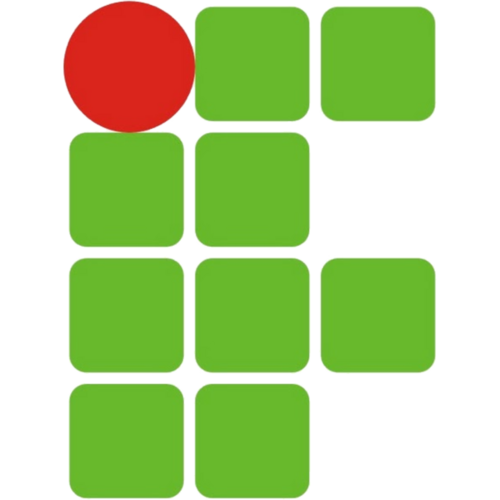
\includegraphics[scale=0.2]{img/IFRN}
	\titlepage
\end{frame}

\logo{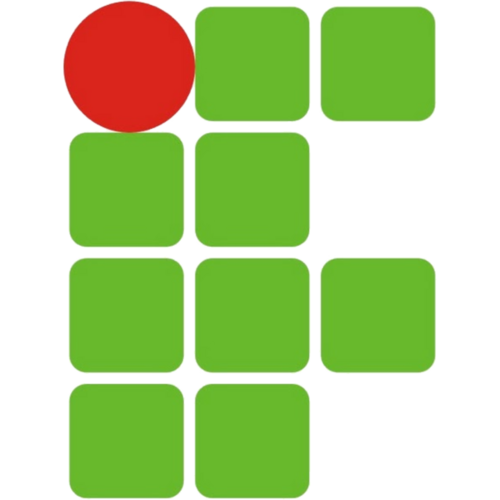
\includegraphics[scale=0.1]{img/IFRN}}

\begin{frame}
	\frametitle{Ementa do Curso}
  	\tableofcontents
\end{frame}

\AtBeginSection[]{
	\begin{frame}
		\frametitle{Ementa do Curso}
		\tableofcontents[currentsection]
	\end{frame}
}

\section{Introdução}

\begin{frame}
	\frametitle{Python}

	\begin{block}{Definição}
		É uma linguagem de script de propósito geral, podendo ser usada para criar
		qualquer tipo de software.
	\end{block}\vfill
	
	\begin{itemize}
		\item Foi concebido no final de 1989 por Guido van Rossum; e
		\item O nome Python teve a sua origem no grupo humorístico britânico
		Monty Python.
	\end{itemize}
\end{frame}

\begin{frame}
\frametitle{Características}

\begin{itemize}
	\item É uma linguagem interpretada;
	\item Os tipos das variáveis são determinados dinamicamente;
	\item Oferece tipos de alto nível;
	\item É orientada a objetos; e
	\item É multi-plataforma.
\end{itemize}
\end{frame}

\begin{frame}
\frametitle{Programa em Python}

\begin{itemize}
	\item Um programa em Python pode ser escrito em qualquer editor de texto;
	\item O documento com o código fonte deve ser salvo com extensão \structure{.py};
	\item Para facilitar o desenvolvimento é comum utilizar-se um IDE
	(Integrated Development Environment); e
	\item O IDLE é o ambiente de desenvelvimento padrão.
\end{itemize}
\end{frame}

\section{Estrutura de um programa}

\begin{frame}[fragile]
\frametitle{Instrução de Saída}

\begin{block}{Definição}
	A instrução de saída de dados é a instrução através da qual o computador se comunica com usuário durante a execução do programa. Isso é feito, geralmente, através da exibição de alguma informação na tela.
\end{block}\vfill

\begin{itemize}
	\item Em Python existe apenas um comando para instrução de saída: \structure{print}.
\end{itemize}\vfill

\begin{exampleblock}{Exemplo}
\begin{lstlisting}
print('Oi, mundo!')
\end{lstlisting}
\end{exampleblock}
\end{frame}

\begin{frame}[fragile]
\frametitle{Comentário}

\begin{block}{Definição}
É uma estrutura da linguagem que permite ao desenvolvedor fazer uma breve explicação do código escrito.
\end{block}\vfill

\begin{itemize}
	\item Comentários são iniciados com \structure{\#}.
\end{itemize}\vfill

\begin{exampleblock}{Exemplo}
	\begin{lstlisting}
# Descrição da funcionalidade desenvolvida
# Autor : Diego
print ('Testando!')
	\end{lstlisting}
\end{exampleblock}\vfill

\begin{alertblock}{Importante}
O que for escrito no bloco de comentário será ignorado pelo interpretador.
\end{alertblock}
\end{frame}

\section{Variável}

\begin{frame}
\frametitle{Variável}

\begin{itemize}
	\item Uma variável representa uma posição de memória;
	\item Possui um nome e tipo;
	\item Seu conteúdo pode variar ao longo do tempo, durante a execução do
	programa;
	\item Embora uma variável possa assumir diferentes valores, ela só pode
	armazenar um valor a cada instante;
	\item Não existe limite para o número de variáveis em um programa; e
	\item Cada variável criada ocupa um espaço de memória de acordo com seu
	tipo e seu tamanho.
\end{itemize}

\end{frame}

\begin{frame}[fragile]
\frametitle{Declaração de Variável}

\begin{itemize}
	\item A tipagem de Python é dinâmica;
	\item Logo não é necessário declarar os tipos de variáveis;
	\item Devem ser declaradas inicialmente por letras $(a - z, A - Z)$ ou sublinhado (\_);
	\item Acentuação é permitida (\alert{não é recomendado}); e
	\item É case sensitive $(a \neq A)$.
\end{itemize}\vfill

\begin{exampleblock}{Exemplos}
	\begin{lstlisting}	
i
nome
data_nascimento
nota1
_sexo
mediaGeral
	\end{lstlisting}
\end{exampleblock}
\end{frame}

\begin{frame}[fragile]
\frametitle{Tipos de Variável}

\begin{itemize}
	\item \structure{str} : Cadeia de caracteres;
	\item \structure{int} : Inteiro;
	\item \structure{float} : Ponto flutuante ou real; e
	\item \structure{bool} : Lógico ou booleano.
\end{itemize}\vfill

\begin{exampleblock}{Exemplos}
\begin{lstlisting}
type('Python')
type(36)
type(82.5)
type(True)
\end{lstlisting}
\end{exampleblock}
\end{frame}

\begin{frame}[fragile]
\frametitle{Operador de Atribuição}

\begin{block}{Definição}
O comando de atribuição é utilizado para conceder valores ou operações a variáveis.
\end{block}\vfill

\begin{itemize}
	\item Em python o operador de atribuição é o sinal de igual: \structure{=};
	\item Do lado esquerdo ao operador de atribuição fica a variável à qual está
	sendo atribuído o valor; e
	\item A direita do operador pode-se escrever qualquer expressão (constantes,
	variáveis ou expressões numéricas).
\end{itemize}\vfill

\begin{exampleblock}{Exemplos}
	\begin{lstlisting}
linguagem = 'Python'
idade = 36
altura = 82.5
matriculado = True
	\end{lstlisting}
\end{exampleblock}
\end{frame}

\begin{frame}[fragile]
\frametitle{Instrução de Entrada}

\begin{block}{Definição}
É o meio pelos quais os dados são transferidas pelo usuário ou pelos níveis secundários de memória ao computador.
\end{block}\vfill

\begin{itemize}
	\item Python possui o comando para instrução de entrada via teclado: \structure{input()}.
\end{itemize}\vfill

\begin{exampleblock}{Exemplo}
	\begin{lstlisting}
nome = input('Digite seu nome:')
print('Oi,',nome)
	\end{lstlisting}
\end{exampleblock}
\end{frame}

\begin{frame}[fragile]
\frametitle{Operadores Aritméticos}

\begin{block}{Definição}
A aritmética é o ramo da matemática que lida com números e com as operações possíveis entre eles.
\end{block} \vfill

 \begin{columns}[c]

\column{.4\textwidth}

\begin{itemize}
	\item \structure{+} : Adição;
	\item \structure{-} : Subtração;
	\item \structure{*} : Multiplicação;
	\item \structure{/}  : Divisão;
	\item \structure{//}  : Divisão inteira;
	\item \structure{\%} : Resto; e
	\item \structure{**} : Potência.
\end{itemize}\vfill

\column{.5\textwidth}
\begin{exampleblock}{Exemplo}
	\begin{lstlisting}
a = int(input('Digite um nú mero inteiro:'))
b = int(input('Digite um nú mero inteiro:'))
c = a + b
print ('Resultado =',c)
	\end{lstlisting}
\end{exampleblock}
\end{columns}
\end{frame}

\begin{frame}[fragile]
\frametitle{Expressão Aritmética}

\begin{block}{Definição}
Uma expressão constitui-se em um conjunto de variáveis e/ou valores, separados por caracteres especiais, que indicam as operações que devem ser executadas.
\end{block} \vfill

 \begin{columns}[c]

\column{.5\textwidth}
\begin{alertblock}{Importante}
Os operadores devem obedecer uma ordem de precedência:
\begin{itemize}
	\item Parênteses;
	\item Potenciação;
	\item Multiplicação, Divisão e Resto; e
	\item Adição e subtração.
\end{itemize}
\end{alertblock} \vfill

\column{.4\textwidth}
\begin{exampleblock}{Exemplo}
	\begin{lstlisting}
a = 2
b = 8
c = a + b / 2
print(c)
	\end{lstlisting}
\end{exampleblock}
\end{columns}
\end{frame}

\section{Estrutura de Seleção}

\begin{frame}[fragile]
\frametitle{Estrutura de Seleção}

\begin{block}{Definição}
Também citado na literatura por Estrutura Condicional, é a
representação de um ou mais comandos de decisão que são responsáveis por mudar o fluxo das instruções de um algoritmo em tempo de execução.
\end{block} \vfill

\begin{itemize}
	\item Python possui apenas uma estrutura de controle: \structure{if}
\end{itemize}

\begin{exampleblock}{Exemplo}
	\begin{lstlisting}
status = 0
if status == 0:
   print('Livre')
else:
   print('Ocupado')
\end{lstlisting}
\end{exampleblock}\vfill

\begin{alertblock}{Importante}
O comando \structure{else} não é obrigatório.
\end{alertblock}
\end{frame}

\begin{frame}[fragile]
\frametitle{Operadores Relacionais}

\begin{block}{Definição}
	Os operadores relacionais estabelecem uma relação entre seus operandos.
\end{block} \vfill

\begin{itemize}
	\item \structure{==} : igual;
	\item \structure{!=} : diferente;
	\item \structure{<} : menor;
	\item \structure{<=} : menor ou igual;
	\item \structure{>} : maior; e
	\item \structure{>=} : maior ou igual.
\end{itemize}\vfill

\begin{exampleblock}{Exemplo}
	\begin{lstlisting}
numero = int(input('Digite um número:'))
if numero >= 0:
    print('Número positivo')
else:
    print('Número negativo')
	\end{lstlisting}
\end{exampleblock}

\end{frame}

\begin{frame}[fragile]
\frametitle{Operadores Lógicos}

\begin{block}{Definição}
Os operadores lógicos definem as maneiras como as relações podem ser conectadas.
\end{block} \vfill

\begin{itemize}
	\item \structure{not} : negação lógica;
	\item \structure{and} : e lógico; e
	\item \structure{or} : ou lógico.
\end{itemize}\vfill

\begin{exampleblock}{Exemplo}
	\begin{lstlisting}
nota = float(input('Digite uma nota:'))
if (nota >= 0) and (nota < 11):
    print('Nota válida')
else:
    print('Nota inválida')
	\end{lstlisting}
\end{exampleblock}
\end{frame}

\begin{frame}
\frametitle{Tabela-verdade}

\begin{exampleblock}{Exemplo}
	\begin{center}
\begin{tabular}{|c|c|c|c|c|}
\hline a = & b = & a \structure{and} b & a \structure{or} b & \structure{not} a\\ \hline
True & True & True & True & False\\ \hline
True & False & False & True & False\\ \hline
False & True & False & True & True\\ \hline
False & False & False & False & True\\ \hline
\end{tabular}
	\end{center}
\end{exampleblock}
\end{frame}

\begin{frame}[fragile]
\frametitle{Estrutura de Seleção Aninhada}

\begin{block}{Definição}
É uma estrutura para desvio de fluxo do programa formada pelo comando de decisão \structure{if} / \structure{elif} / \structure{else} mais subestruturas de decisão.
\end{block}\vfill

\begin{exampleblock}{Exemplo}
\begin{lstlisting}
numero = int(input('Digite um número inteiro:'))
if numero > 0:
    print ('Número positivo')
elif numero < 0:
    print ('Número negativo')
else:
    print ('O número digitado foi zero')
\end{lstlisting}
\end{exampleblock}
\end{frame}

\section{Estruturas de Repetição}

\begin{frame}
\frametitle{Estruturas de Repetição}

\begin{block}{Definição}
Uma estrutura de repetição é uma estrutura de desvio do fluxo de controle presente em linguagens de programação que realiza e repete diferentes computações ou ações.
\end{block}\vfill

\begin{itemize}
\item Python possui duas estruturas de repetição:
\begin{itemize}
	\item \structure{while}; e
	\item \structure{for}.
\end{itemize}
\end{itemize}
\end{frame}

\begin{frame}[fragile]
\frametitle{Estrutura While}

\begin{block}{Definição}
A construção while (também chamada repetição pré-testada) é a mais difundida estrutura de repetição.
\end{block}\vfill

\begin{exampleblock}{Exemplo}
\begin{lstlisting}
i = 1
while i <= 10:
    print (i)
    i = i + 1
\end{lstlisting}
\end{exampleblock}
\end{frame}

\begin{frame}[fragile]
\frametitle{Comando Break}

\begin{block}{Definição}
O comando \structure{break} permite parar uma execução de uma instrução de repetição toda vez que o mesmo for invocado, ignorando, caso ainda existam, outras instruções a serem executadas.
\end{block}\vfill

\begin{exampleblock}{Exemplo}
	\begin{lstlisting}
i = 1
while i <= 10:
    print (i)
    if i == 5: 
        break
    i = i + 1
	\end{lstlisting}
\end{exampleblock}
\end{frame}

\begin{frame}[fragile]
\frametitle{Estrutura For}

\begin{block}{Definição}
A construção \structure{for}, ou repetição com variável de controle, é uma estrutura de repetição que designa uma variável de controle para cada iteração do bloco, e uma operação de passo a cada iteração.
\end{block}\vfill

\begin{exampleblock}{Exemplo}
	\begin{lstlisting}
for i in range(11):
    print(i)
	\end{lstlisting}
\end{exampleblock}
\end{frame}

\section{Subprograma}

\begin{frame}
\frametitle{Função}

\begin{block}{Definição}
São subrotinas (módulos ou métodos) de programas, capazes de executar uma tarefa definida pelo programador, que pode retorna ou não algum valor. Os programas desenvolvidos com subprogramas são ditos modulares.
\end{block} \vfill

\begin{itemize}
	\item Python possui uma estrutura para definição de função: \structure{def}.
\end{itemize}
\end{frame}

\begin{frame}[fragile]
\frametitle{Função}

\begin{exampleblock}{Exemplo 1}
	\begin{lstlisting}
def mensagem():
    print('Oi , mundo!')

mensagem()
	\end{lstlisting}
\end{exampleblock}\vfill

\begin{exampleblock}{Exemplo 2}
	\begin{lstlisting}
def somar(a,b):
    return a + b

valor1 = float(input('Digite o primeiro valor :'))
valor2 = float(input('Digite o segundo valor :'))
resultado = somar(valor1,valor2)
print('A soma de ',valor1 ,' + ',valor2 ,' = ',resultado)
	\end{lstlisting}
\end{exampleblock}
\end{frame}

\begin{frame}[fragile]
\frametitle{Recursão}

\begin{block}{Definição}
É quando uma função refere-se a si própria durante a própria definição.
\end{block} \vfill

\begin{exampleblock}{Exemplo 2}
\begin{lstlisting}
def contador(i):
    if i > 1:
        contador(i - 1)
    print (i)

contador(10)
\end{lstlisting}
\end{exampleblock}
\end{frame}

\end{document}